\chapter{INTRODUCTION}

{\baselineskip=2\baselineskip

\section{Background of the Study}

\textit{Theobroma cacao}, widely known as cacao, is one of the most economically influential crops in the world. It serves as the primary raw material for the multibillion-dollar chocolate industry, supporting the livelihoods of approximately six million small-scale farmers globally. Once harvested, cacao seeds are processed to produce cocoa powder and cocoa butter—essential ingredients used in a wide range of products, from confections and beverages to cosmetics and pharmaceuticals. Despite its global demand and economic importance, cacao cultivation faces persistent challenges from various biotic and abiotic stressors. In particular, fungal pathogens such as \textit{Phytophthora palmivora} cause black pod disease, which has been documented to inflict significant annual yield losses \cite{Avila2023}.

Traditional disease management in cacao farms typically involves manual inspection and subjective classification of pods. The \cite{PhilCacaoRoadmap2021} reported that this method is labor intensive and error prone, often failing to detect infections in their early stages—especially in regions with limited access to skilled agricultural labor and advanced diagnostics. In the Philippines, for example, cacao production has not kept pace with local consumption demands. Despite favorable growing conditions, the Davao Region has been recognized as the ``Cacao Capital of the Philippines'' \cite{PCAF2021}.

To address these threats, modern agriculture has increasingly turned to advanced technological solutions for early disease detection and intervention. Unmanned Aerial Vehicles (UAVs) and deep learning algorithms have emerged as powerful tools in precision agriculture, offering efficient and scalable monitoring of large plantations. UAVs, equipped with high-resolution cameras and multispectral sensors, can rapidly survey wide areas, while cutting-edge models like You Only Look Once (YOLO) provide high-accuracy plant disease identification \cite{Vyas2023}. Early detection during the pre-harvest phase, as supported by \cite{Upadhyay2025,Yadav2024}, enables timely interventions to mitigate crop losses and ensure quality harvests.

Existing technological interventions for cacao disease detection, such as mobile applications that utilize image processing and machine learning, have made strides in bridging the gap. For instance, \cite{Tan2018} developed AuToDiDAC, an app designed to detect black pod rot, while \cite{Tovurawa2025} used convolutional neural networks (CNNs) to classify cacao leaf diseases. However, these solutions are predominantly dependent on static image inputs and close-range data collection. As noted by \cite{Taesiri2023}, such methods can cause models to focus only on the most discriminative regions of the plant, potentially missing early-stage infections or atypical symptoms that may be spread across the pod’s surface. Additionally, mobile-based approaches require farmers to manually photograph individual pods, which is laborious and impractical for large-scale plantations, thereby limiting mobility and scalability.

With these challenges in mind, this study introduces a UAV-based cacao disease detection system that leverages aerial imagery and the YOLO object detection algorithm to overcome the constraints of static, close-range data collection. By capturing images from various angles and altitudes, this approach enables more comprehensive monitoring of cacao plantations. Integrating deep learning models with UAV technology allows for the detection of disease symptoms across the entire pod surface that traditional methods may miss.

The system will be developed and followed by field tests to evaluate its performance, functionality, and integration in real-world agricultural environments. Its potential for large-scale deployment in cacao farms will also be assessed, aiming to provide a scalable, efficient, and accurate disease detection solution for one of the world’s most valuable crops.

\section{Statement of the Problem}

The Philippine cacao industry faces persistent challenges that hinder its ability to meet the demands of both the domestic and international market. Although the country has favorable climate conditions and fertile land, especially in the Davao Region, which represents 78\% of national production, it continues to fall short of its annual production target of 50,000 metric tons. According to the \cite{PhilCacaoRoadmap2021}, this shortfall is largely due to cacao diseases, particularly black pod disease caused by \textit{Phytophthora palmivora}, which leads to post-harvest losses of up to 90\%.

Traditional detection methods rely on manual inspection, which is labor intensive, slow, and prone to human error, leading to delayed intervention and significant crop losses. Although existing studies explore machine learning and imaging technologies for cacao disease detection, they primarily use static imaging and mobile-based approaches, limiting monitoring and scalability. To address this gap, this study proposes the integration of an Unmanned Aerial Vehicle (UAV) with You Only Look Once (YOLO) technique for detection of cacao pod disease, particularly \textit{Phytophthora palmivora}, without human effort. The system also includes geotagging, using QGIS to pinpoint where the affected cacaos are, which are processed and viewed in a web-based application where farmers can monitor their cacao farms.

\section{Objectives of the Study}

This study aims to design a UAV-based system that integrates object detection model for identifying \textit{Phytophthora palmivora} disease in cacao pods, with GPS geotagging for precise location mapping. Specifically, it seeks to:

\begin{enumerate}
	\item Design and configure a UAV capable of autonomous navigation over cacao farms while providing stable flight and imaging.
	\item Develop and implement a monitoring system that tracks the UAV’s flight status and detection for cacao pod disease.
	\item Implement a object detection model for cacao pod detection and a classification model for identifying \textit{Phytophthora palmivora} infection.
	\item Test the system’s detection accuracy, classification performance, geotagging precision, and overall operational efficiency.
\end{enumerate}

\section{Significance of the Study}

This study holds significance for multiple sectors, starting with cacao farmers, who will benefit from a practical and accessible solution for early disease detection, enabling timely intervention to prevent further contamination. This proactive approach helps reduce crop losses, improve yield quality and quantity, and promote stable income and long-term sustainability in farming practices.

The cacao and chocolate industry will also gain from a more disease-resilient cacao supply, ensuring stability and reliability in the value chain, supporting both local and global markets, and maintaining consistent raw material availability to sustain production, control prices, and boost economic activity in cacao-dependent regions. For the agricultural sector, the system promotes the modernization of farming through precision agriculture technologies, enhancing productivity and sustainability, particularly in disease-prone areas.

The government can leverage the study’s outcomes to align with national agricultural development goals, such as those in the Philippine Cacao Industry Roadmap, providing a basis for policy-making, funding assistance, and technology-based interventions, while contributing to Sustainable Development Goals (SDG 8 and SDG 15) by fostering sustainable agriculture, increasing farmer income, and encouraging innovation. Lastly, future researchers in precision agriculture and remote sensing can use this work as a valuable reference for further advancements in plant disease detection technologies.

\section{Scope and Limitations}

This study focuses on the development and testing of a UAV-based detection system for cacao farms in Claveria, Misamis Oriental. The system integrates three major components: (1) a YOLO-based model for detecting symptoms of \textit{Phytophthora palmivora} infection in cacao pods, (2) GPS and QGIS for precise geolocation and mapping of affected areas, and (3) a web-based application for monitoring and visualization of results.

The scope of the system is limited to the detection of external symptoms of black pod disease, such as visible pod rot. Internal infections that are not outwardly visible cannot be identified by the current implementation. Furthermore, while the system can assist in identifying potentially infected pods, it does not automate subsequent farm management activities such as pruning or removal of diseased pods, which must still be performed manually by farmers.

The imaging capability of the UAV is also constrained by the use of a 720p camera, which may affect the level of detail captured and thus the accuracy of disease detection under certain conditions. Additional environmental factors such as lighting, weather conditions, and UAV flight stability may also influence detection performance. These limitations define the operational boundaries of the proposed system and provide considerations for future improvements.

\section{Conceptual Framework}

\begin{figure}[H]
	\centering
  \caption{IPO Model}
	\label{fig:ipo}
	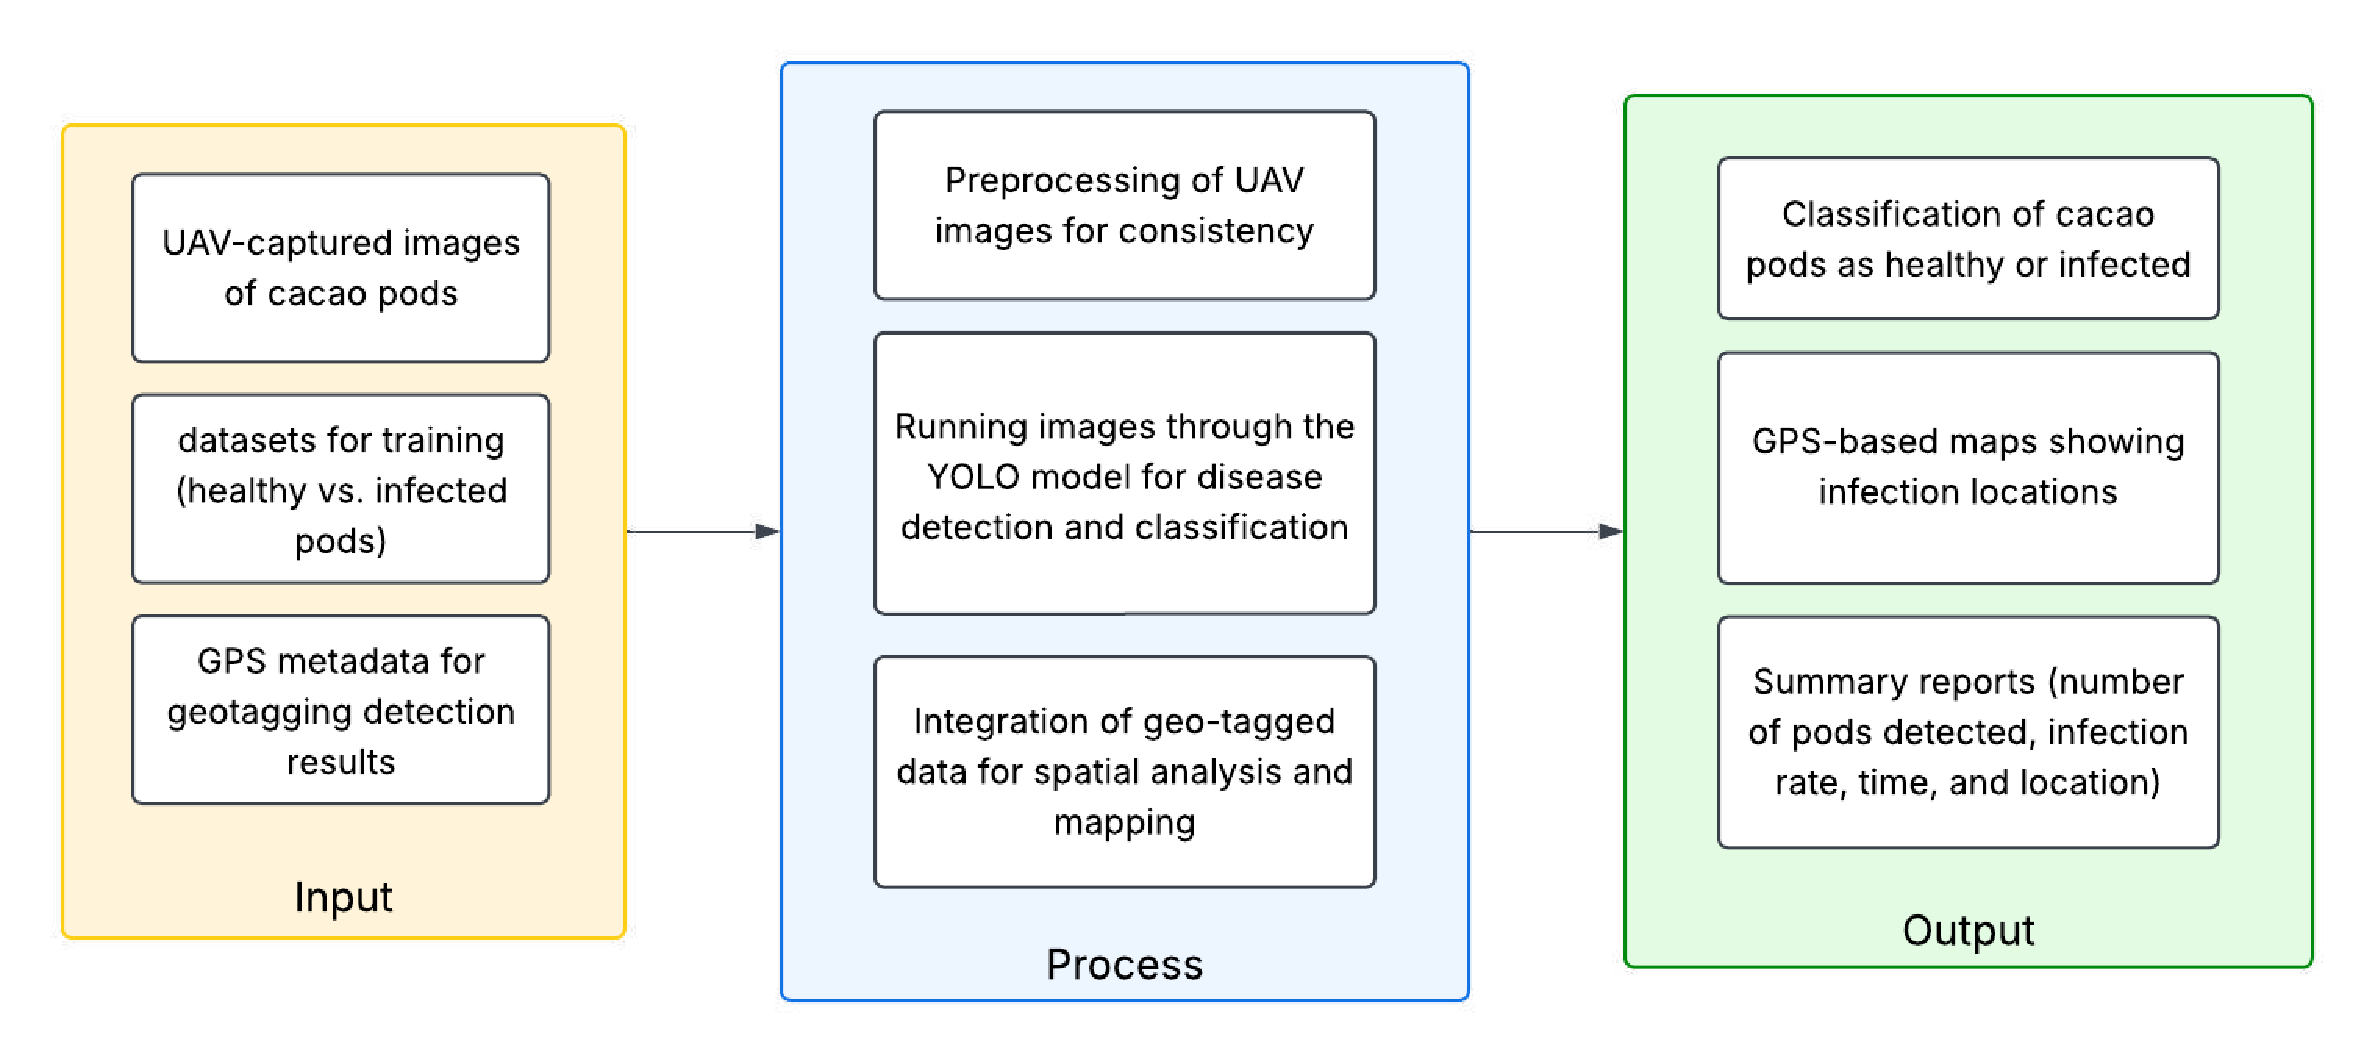
\includegraphics[width=1\textwidth]{figures/IPO.pdf}
\end{figure}

The study's conceptual framework is presented through an Input-Output-Process Model. The process begins with the input stage, where drones are used to capture images of cacao pods in the farm. These images serve as the primary source of information and are compared with sets of sample images showing both healthy and diseased pods. Along with the images, location data is recorded so that each detection can be linked to its exact place in the farm. At this stage, farmers also provide feedback on how easy the system is to use and how accurate it appears, ensuring that the design reflects their real needs.

The information collected then moves to the process stage. Here, the pod images are first checked to make them clear and consistent for analysis. After this, the system studies the images to identify whether pods are healthy or show signs of disease. The location data gathered during drone flights is combined with the results, allowing the system to create maps that show the areas where diseases may be present. This stage transforms raw images into useful information that can guide farmers in managing their crops.

In the output stage, the system produces results that are directly useful for farm management. These include the classification of cacao pods as healthy or infected, maps that point out exactly where the infected pods are located, and summary reports. The reports provide details such as the total number of pods detected, the percentage that are infected, and the specific times and places where infections were found.


\section{Definition of Terms}

For clarity and consistency, the following terms are defined as they are used in this study:

\begin{description}
	\item[Dataset] - A structured collection of related data, such as images of cacao pods, used to train and evaluate deep learning models for disease detection in this study.

	\item[Deep Learning Algorithms] - A subset of machine learning algorithms, particularly neural networks, used to analyze large datasets and recognize patterns in images or other inputs, enhancing precision agriculture applications.

	\item[Disease Detection] - The process of identifying and diagnosing plant diseases, often involving technology such as image analysis and machine learning algorithms for early intervention.

	\item[Field Tests] - Practical trials conducted in real-world agricultural environments to assess the effectiveness and performance of the proposed UAV and deep learning-based system for detecting cacao pod diseases.

	\item[Geotagging] - The process of adding geographical location data, such as latitude and longitude, to images or data collected by UAVs, enabling spatial tracking and mapping of disease occurrences in cacao farms.

	\item[Image Processing] - The technique of manipulating and analyzing digital images using algorithms to extract meaningful information, often for detecting patterns such as plant diseases.

	\item[\textit{Phytophthora palmivora}] - A fungal pathogen responsible for causing black pod disease in cacao plants, which leads to significant yield losses in cacao production.

	\item[Pod] - Refers to the fruit of the cacao tree that contains cacao beans; it is the primary site for disease detection, particularly for symptoms caused by pathogens like \textit{Phytophthora palmivora}.

	\item[Pre-harvest Detection] - The process of identifying signs of disease or stress in crops, specifically cacao pods, before they are harvested, allowing for timely intervention to prevent yield loss and improve crop quality.

	\item[QGIS] - An open-source Geographic Information System software that provides tools for geospatial data processing, mapping, and analysis. In this study, it is used for automating geotagging and visualizing infected cacao trees.

	\item[Static Imaging] - The process of capturing fixed, non-moving images, often used in traditional disease detection methods, which may miss early-stage infections or dispersed symptoms.

	\item[Unmanned Aerial Vehicles (UAVs)] - Aerial devices, typically drones, that operate without a human pilot, often equipped with cameras and sensors, used for monitoring agricultural environments and gathering data for analysis.

	\item[You Only Look Once (YOLO)] - An advanced real-time object detection model that can quickly identify and classify objects within images, used for detecting diseases on plant surfaces in this study.
\end{description}
